\documentclass{article}
\usepackage{indentfirst}
\usepackage{graphicx} % Required for inserting images
\usepackage{wrapfig}
\usepackage{geometry}
\usepackage{cite}
\newgeometry{vmargin={15mm}, hmargin={30mm,30mm}}
\title{TDPS Initial Report\\Team-07}
\author{
2613968Z\ Zou Hanlin\\
\and
2614344G\ Gu Xingci\\
\and
2613973G\ Guo Linhong\\
\and
2613949C\ Chen Xi\\
\and
2613977S\ Sun Linhan\\
\and
2613977S\ Liu Cehan\\
\and
2613951L\ Li Chenghao\\
\and
2614354Y\ Yang Chun\\
\and
2614329S\ Sheng Dian\\
\and
2614353Y\ Yuan Ye}
\date{March 2023}

\begin{document}

\maketitle
%The initial/first design report should include your system-level approach and design idea that you have decided to implement in your hardware/software development to execute the given tasks on both patios. You can present your proposed system-level design either as a block diagram or flowchart. Your report should also include the rationale (discussion/reasons) behind the chosen sensors, system design and integration approaches. During our meeting, I will be more interested in knowing why you selected particular sensors and decided to build your autonomous robot/car based on the presented system design. This initial design report should not contain more than 1500 words and should not be longer than 3-pages, these include words, diagrams, figures, and charts. The cover page does not count as part of the 3-page limit.
%the report should be formal detailing your design methodology
\begin{abstract}
%Put abstract here
The team design project requires 10 team members to design, build and present a rover that accomplishes activities on East Lake, UESTC, with two patios, each containing three tasks. Our original designed rover is equipped with an OpenMV camera, three ultrasonic detectors as its sensors, Nucleo-H7 as the central controller, a single robotic arm, a servo and others. These have form a unified system in the top-level system design flowchart, which is initially subdivided into sensor design, control design, and integration design. Our rover could accomplish the preliminary completion of the six tasks.
\end{abstract}
\newpage

\section{Introduction}
Intelligent small rover is a prominent topic of research. It has a chassis, wheels, motor, micro controller, and battery pack. It avoids impediments and drives independently using sensors, controls, and algorithms~\cite{92}.

In this course, we build an autonomous rover that can complete three tasks on each of the two patios at East Lake of UESTC.

The remainder of this paper proceeds as follows. Section 2 discusses functions of rover. Section 3 creates a rover system flowchart. Sections 4, 5, and 6 present rover sensor, control, and integration designs. In Section 7 the report is concluded and future improvement is given.

\section{Task Analysis}
% The design of the robot is based on its functions, which is defined by the tasks given in the course handbook. 
% Mecanum wheels are designed to be installed on the chassis of the robot to make it move in the patio. A servo with a 3D-printed robotic arm is going to be used to release the ball to the basket. To drive these wheels and the servo, a STM32 micro controller is going to be programmed. 
% To follow the curve on the ground in the patio and to read the instructions given by shape(patio 2 task1), the robot needs a OpenMV camera to analysis. Ultrasonic distance sensors are also going to be used to detect the barrier at the front and rears on the robot.
% To send the radio signal containing names of team member and current time, a RTC (Real Time Clock) and a pair of HC12 radio models are needed.
    \subsection{Patio1}
    To perform tasks 1.1 and 1.3, where the rover must follow colorful tiles and stop at a gate, OpenMV needs to have visual identification and pavement processing capabilities to determine the optimal route. Task 1.2 involves locating and crossing a bridge, requiring three ultrasonic detectors to ensure proper alignment with the bridge and sidewall.
    
    \subsection{Patio2}
    Task 2.1 involving identifying arrow shapes and directions, the OpenMV camera in patio1 must be modified. To complete Task 2.2, a robotic arm attached to the servo is needed to launch a tennis ball into a basket. Task 2.3's main requirement is communication, which involves using a wireless transceiver to send messages to a laptop computer.
    
\section{Top-level System Design}

\begin{wrapfigure}{L}{0.35\textwidth}
    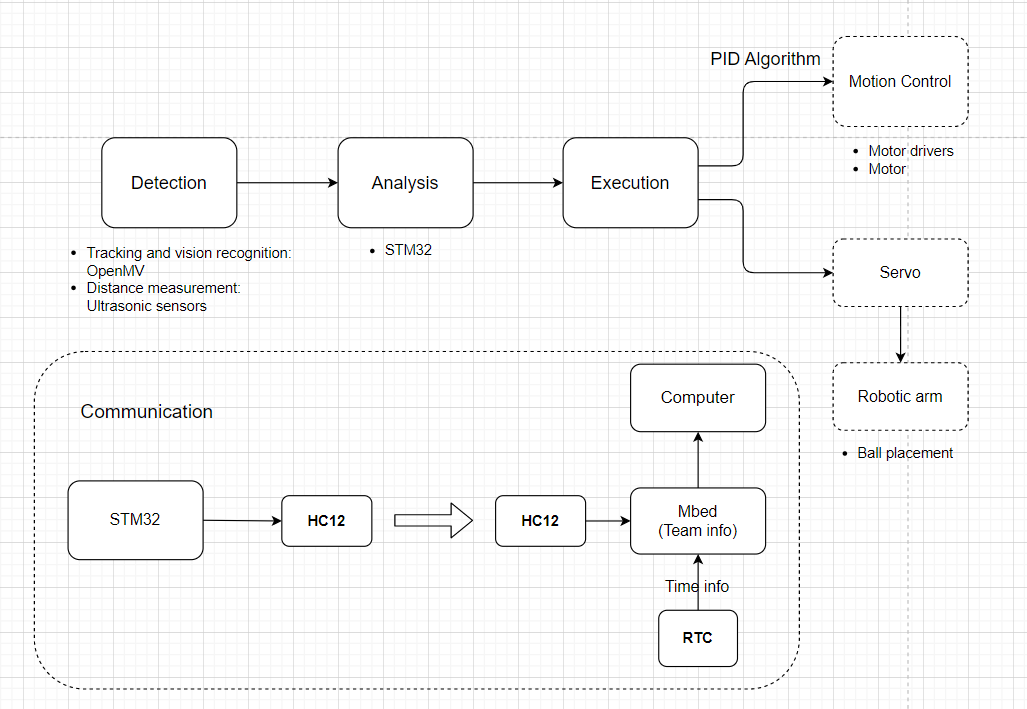
\includegraphics[width=0.33\textwidth]{figure/dia_o.png}
  \caption{System Flowchart}
  \label{diag}
\end{wrapfigure}

The flowchart of the system is shown as Figure~\ref{diag}.

For detection phase, an OpenMV camera and ultrasonic detectors are utilised as sensors to identify the patio tiles and estimate the robot's distance from the handrail.

STM32 MCU receives information gathered by sensors for analysis. At the execution part, a servo is instructed to drop the ball into the hoop via a mechanical arm, and stable functioning of the Mecanum wheels is controlled by PID algorithm~\cite{pid} .

In the communication section, an HC12 module is activated to transmit team information together with the current time given by an RTC module.

\section{Sensor Design}
The sensor module detects physical parameters, sends data to the car's control system, and helps the rover adjust its behavior.

    \subsection{OpenMV Camera Programming Design}
    
        \subsubsection{Edge detection}
        Rover must navigate a scarce gravel pavement and a flat stone pavement. Canny operator is selected to acquire the thick and intricate patrol pavement edge and the sparse standard pavement edge.
        
        \subsubsection{Filtering, Adaptive binarized image}
        The Mean operator blurs the image in order to reduce the following computing burden. Then, use mean pooling on gray scale images to detect pavement only in pixels with dense edges.
        
        \subsubsection{Arrow identification}
        Traditional digital image processing methods are able to extract the geometrically weighted centre of the arrow, but are unable to identify it from a distance. Machine learning was chosen in the end, photographing acrylic standing plates beside black standing plates, manually labelling them, then cropping the model with Edge Impulse to determine arrow direction.
        
    \subsection{Ultrasonic sensors design}
        \subsubsection{Distance Measurement}
        Three ultrasonic detectors are going to be installed, and two of them would be installed parallel to the rover’s right side at railing column height. The front ultrasonic detector measures the distance to the bridge, while the side sensors measure two lengths to make sure it's parallel to the bridge and side wall to complete task 1.2.
        
        \subsubsection{Navigation}
        During the basket searching process, it is planed to use multiple ultrasonic detectors to ensure that the rover can navigate stably along the railing's edge, as the cobblestone texture on the ground is difficult to extract reliably to find the trash can.
        
\section{Control Design}
The control module employs the PID algorithm~\cite{pid} to control the motors, and controls the servo-controlled robotic arm with a PWM output.

    \subsection{Chassis Design}
    
        \subsubsection{Motor Control}
        Basic motor control is driven by a PWM output to alter the duty cycle, consequently adjusting the output size to control the motor speed, and changing the voltage of the two digital pins, high and low, to control the direction of the motor.
        
        \subsubsection{PID Adjustment}
        As the PID concept is simple, robust, and applicable, it significantly enhances the accuracy of wheel movement. In our rover, we employ the PID algorithm to verify that the actual speed of the wheel corresponds to the necessary speed.
        
        \subsubsection{UART Communication}
        UART communication is characterized by receiving host controller-sent messages. This communication from the host controller handles and allocates the speeds and directions of four Mecanum wheels by receiving data from an OpenMV camera.
    
    \subsection{Robotic arm design}
    
        \subsubsection{Servo}
        One MG995 servo, a metal servo that rotates more forcefully and steadily than average servos, is used to drive the robotic arm. A PWM signal activates the servo, which rotates the arm for 180 degrees from its initial position and drops the ball into the basket.
        
        \begin{wrapfigure}{L}{0.35\textwidth}
            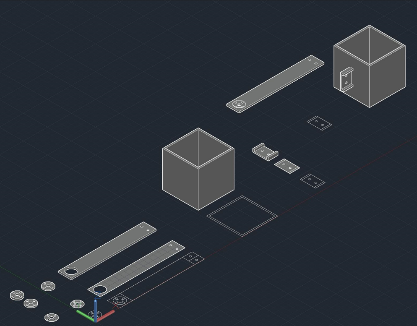
\includegraphics[width=0.33\textwidth]{figure/3dprint.png}
          \caption{Parts of the robotic arm}
          \label{3d}
        \end{wrapfigure}
        
        \subsubsection{Robotic Arm}
        
        The 3D model of the robotic arm is shown as Figure~\ref{3d}.
        
        The robotic arm is designed using 3D modelling and printing, allowing the adjustment of the length, thickness, and interface type of the driving rod. The robotic arm transmission rod is on the right, while the robotic arm disc is on the left. The right side is attached to the pool table's frame, the basket and connection are connected by screws and nuts, and 3mm redundant space is reserved at the front and back to reduce jamming and damping.
        
\section{Integration}
Communication approaches and PCB design are the foundation of the Integration design, forming the backbone of the system design, making it robust and efficient.

    \subsection{Communication design}
    
        \subsubsection{Communication Module}
        %意义不明需要重写We choose to use separate design, which split the core control and communication module to reduce memory utilisation and increase time communication stability. As the rover reaches its destination, the main control stm32 (H7 series) sends an enabling signal to the outside through its HC12. The HC12 attached to the Nucleo-L432KC transfers data through UART after receiving the signal.
        HC12 radio module is chosen to transmit information from the rover, which works at a frequency of 433MHz and is controlled by UART. A pair of HC12 are used to transmit data between the rover and the computer.
        
        \subsubsection{Data Sending}
        %意义不明需要重写Since external crystal oscillator module pre-injects Beijing time, we choose DS3231 for RTC. The module clocks without electricity, processing time. After receiving the signal, Nucleo-L432KC reads the time of the DS3231 crystal oscillator module for buffering purposes. The group's name and time are then transmitted to the PC via USB and displayed on the PC.
        As the rover reaches its destination, the main controller STM32 (H7 series) sends an enable signal to the outside through its HC12. The HC12 attached to the Nucleo-L432KC transfers data to the computer through UART after receiving the signal. By using this design, the load of the main controller is lessened and the communication stability is improved. RTC (Real Time Clock)~\cite{rtc} is a module that could provide real time for digital devices. After Nucleo-L432KC receives the enable signal, it would send current time obtained by RTC and team information to the computer by UART.
        
    \subsection{PCB (Printed Circuit Board) Design}
    The PCB serves as a stable connector among components of the system, including battery, sensors, STM32 micro controller, servo, motor drivers and communication module. The specific design of the PCB is going to be done after testing the system.
    
\section{Conclusion}
The rover uses sensor, control, and integration modules to complete six tasks on two patios in this course. Early planning and coordination helped these modules provide a reliable hardware platform for the software to accomplish basic functions. Future enhancements should add ultrasonic sensors to the OpenMV camera's sensor part to stabilise the rover's navigation while finding trash cans in Patio2. For the control design, the robotic arm's tennis ball would fall out after 90 degrees, resulting in an insufficient drop point and requiring improvement.


\bibliographystyle{IEEEtran}
\bibliography{IEEEabrv,references.bib} 

%\subsection{OpenMV pavement inspection}
%The pavement used for  inspection is thin gravel, while the surrounding pavement is flat slate. Judge the current direction of the rover according to the difference between the pavement to be inspected and its surrounding.
%\subsection{Edge detection}
%\begin{figure}[h]
%    \centering
%    \includegraphics[width=0.9\textwidth]{figure/fig2.png}
%    \caption{OpenMV}
%    \label{a}
%\end{figure}
%Canny operator is used to detect the edge of the pavement surface. The results show that the edge of the inspected path surface is dense and complex, while the edge of the normal path surface is sparse. This step needs to detect as many edges as possible, hence a large resolution is needed.
%\begin{figure}[h]
%    \centering
%    \includegraphics[width=0.9\textwidth]{figure/fig1.png}
%    \caption{OpenMV}
%    \label{a}
%\end{figure}
%\subsection{Filtration}
%\begin{figure}[h]
%    \centering
 %   \includegraphics[width=0.9\textwidth]{figure/fig3.png}
  %  \caption{OpenMV}
   % \label{a}
%\end{figure}
%Filtration is applied by using the standard mean of the box filter for fuzzy filtering. The meaning of 5 is that the kernel size is 7x7. The result is a blurred image, with some edges on the surrounding pavement blurred to a point where it is almost impossible to see, while many edges on the inspected pavement blurred to look more like a whole.
%\begin{figure}[h]
 %   \centering
 %   \includegraphics[width=0.9\textwidth]{figure/fig4.png}
 %   \caption{OpenMV}
 %   \label{a}
%\end{figure}

%Using mean pooling, convert each 10x10 size pixel to one pixel in order to reduce the calculation overhead of next step.
%\begin{figure}[h]
 %   \centering
 %   \includegraphics[width=0.9\textwidth]{figure/fig5.png}
 %   \caption{OpenMV}
 %   \label{a}
%\end{figure}
%\subsection{Adaptive image binarization}

\end{document}
